\section{Receiver Eliminate}
\label{pruneReceiver}
In the design option tree, the GLAS branch is obviously dropped out, since we are trying to improve the whole concept. Meanwhile, the \ac{MPD}'s single-photon detection modules branch has different quantum efficiency for different wavelength. Which means MPD can be used as green laser detector with 49\% efficiency but it is eliminated for infrared laser with approximate 1\% efficiency. The 32x32-Pixel Array with In-Pixel Photon Counting could be a new approch since............

The pruned design option tree for the laser detector can be seen in figure \ref{fig:DOTreceiverPruned}.

\begin{figure}
\centering
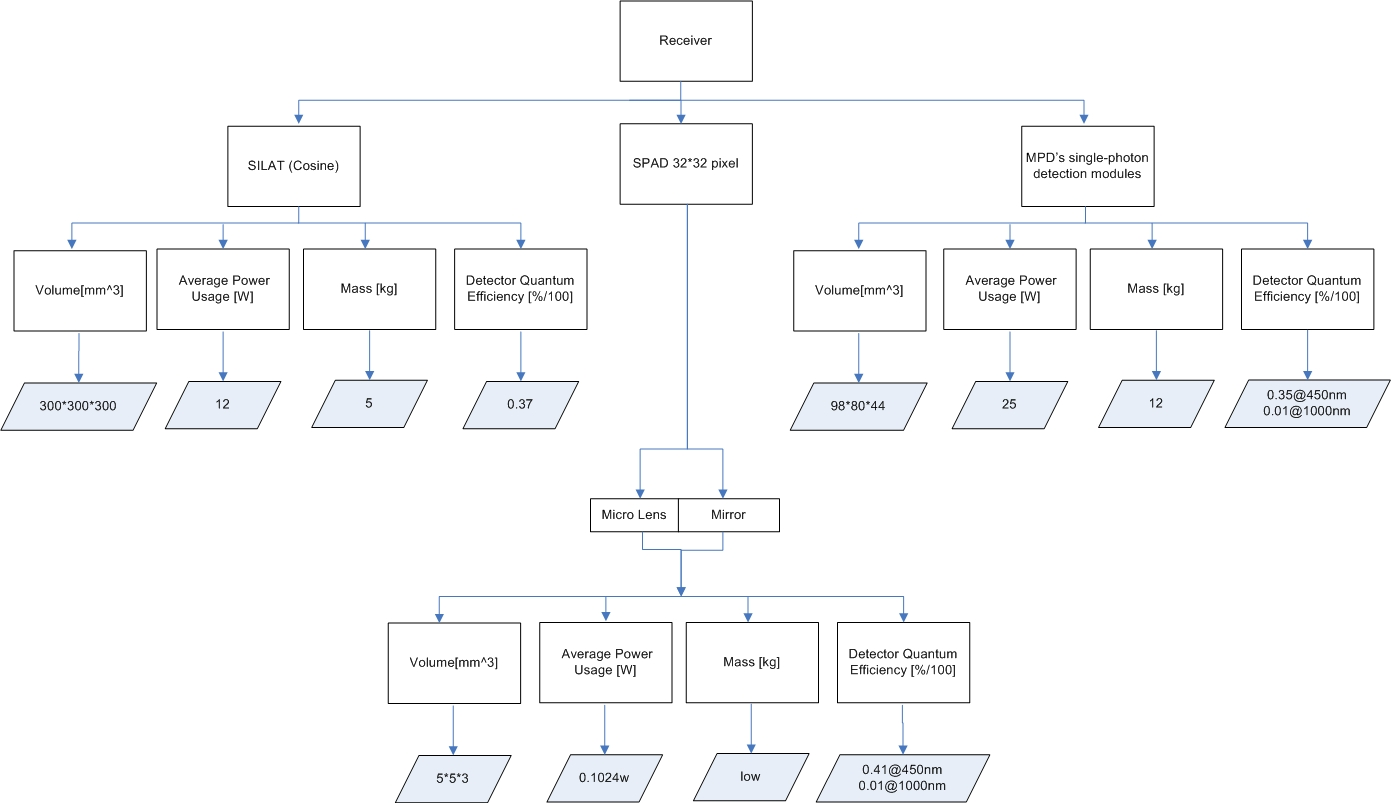
\includegraphics[width=\textheight, angle=90]{chapters/img/DOTreceiverPruned.jpg}
\caption{The pruned design option tree for the Laser receivers}
\label{fig:DOTreceiverPruned}
\end{figure}